
\newcommand{\depBox}[1]{
	\begin{adjustbox}{minipage=0.90\textwidth,margin=0 \smallskipamount,center}
		Abhängigkeiten:	 #1
	\end{adjustbox} ~\\
}

\section{Module}
\subsection{Modulübersicht}
Die Teilbereiche des Projekts wurden in verschieden Module aufgeteilt.

\begin{figure}[h!]
	\centering
	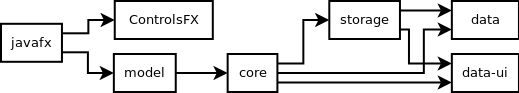
\includegraphics[width=.8\textwidth]{module_dependencies.png}
	\caption{Abhängigkeitsgraph der Module}
	\label{mod_dep_view}
\end{figure}

Der in Abbildung \ref{mod_dep_view} gezeigte Graph enthält keine Abhängigkeiten nach JUnit und
dem JDK aus Gründen der Übersicht. Zudem ist ControlsFX \cite{controlsfx} kein eigen
entwickeltes Modul und wird lediglich aus gründen der Vollständigkeit aufgeführt.

Anzumerken ist auch, dass bis in das \refLongP{\textModCore} keine Abhängigkeiten
gegenüber einer UI-Bibliothek existieren. Das Modul \hyperref[mod_data-ui]{Data-UI} stellt
zwar Komponenten bereit, die für die Integration in eine Benutzeroberfläche benötigt werden,
bleibt jedoch Benutzeroberflächenunabhängig.


\subsection{\textModCore}
\label{\textModCore}
\begin{figure}[h!]
	\centering
	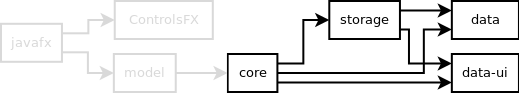
\includegraphics[width=.8\textwidth]{module_dependencies_core.png}
\end{figure}
\depBox{\refLongP{\textModData}, \refLongP{\textModDataUI}, \refLongP{\textModStorage}}

Modulerklräung hier
Core inklusive Abhängigkeiten enthalten alle Logik. Falls eine ander Benutzeroberfläche erstellt,
oder die Logik anderweitig benötigt wird, sollte auf dieses Modul die Abhängigkeit aufgebaut werden.




\subsection{\textModData}
\label{\textModData}
\begin{figure}[h!]
	\centering
	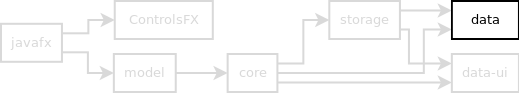
\includegraphics[width=.8\textwidth]{module_dependencies_data.png}
\end{figure}
\depBox{Keine}

Das Modul \textit{data} enthält die Haupt-Geschäftslogik und alle Datenmodelle. Da viel Logik nur darin besteht
die referentielle Integrität bzw. Vollständigkeit der Daten zu gewährleisten ist dieses Modul im Gegensatz zum
Modul \textit{core} relativ schwergewichtig.

\subsubsection{Bindings}
Zur Kommunikation innerhalb dieses Moduls wird größtenteils das ObservableValue-Pattern verwendet. Hierbei wird auf
die Java-eigene Klasse \textit{PropertyChangeSupport} zurückgegriffen. Diese Klasse ermöglicht das Registrieren
von Handlern bzw. das Auslösen von Events. Zudem unterstützt JavaFX diese Art von ObservableValue, wodurch es
möglich ist, im \textit{javafx} Modul Properties von JavaFX mit Properties des Datenmodells zu verbinden. Beispielhaft
sieht eine solche Klasse folgendermaßen aus.

\begin{figure}[h!]
	\centering
	\begin{lstlisting}
public class Bean {
    private final PropertyChangeSupport pcs = new PropertyChangeSupport(this);
    private String name;

    public String getName() {
    	return name;
    }
    public void setName(String name) {
    	String old = this.name;
    	this.name = name;
    	pcs.firePropertyChange("name", old, name);
    }
    public void addPropertyChangeListener(PropertyChangeListener listener) {
    	pcs.addPropertyChangeListener(listener);
    }
}
	\end{lstlisting}
	\caption{Beispiel Java Bean}
\end{figure}

\subsubsection{Flow Notation Parser}
Dieser Parser ist für die Umsetzung von textueller Flow-Notation in eine auswertbare Form zuständig. Hierbei können
beispielsweise folgende Konstruke verarbeitet werden:

\begin{itemize}
	\item \{name:string\}
	\item \{int\}
	\item \{(name:string, amount:int)\}
	\item (name:string)
	\item (float)*
	\item (float*, int)
	\item (float*, int)/(double*, int)
\end{itemize}
Vom Parser wird ein generisches \textit{FlowAction} Objekt zurückgegeben, wenn der Vorgang erfolgreich war. Dieses
Objekt kann eines der folgenden Klassen sein:

\begin{itemize}
	\item MultiStream ( \textbf{\{}test\textbf{\}} )
	\item Tupel ( \textbf{(}test\textbf{)} )
	\item Type ( \textbf{name:test} )
	\item Chain ( \textbf{test/int} )
\end{itemize}
Objekte dieser Klassen enthalten entsprechend Möglichkeiten auf die Kind-Elemente (wenn vorhanden) oder
Eigenschaften zuzugreifen.
\subsection{\textModDataUI}
\label{\textModDataUI}
\begin{figure}[h!]
	\centering
	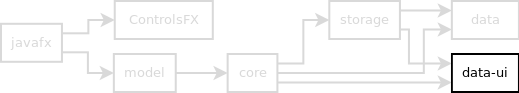
\includegraphics[width=.8\textwidth]{module_dependencies_data-ui.png}
\end{figure}
\depBox{Keine}

Im Modul \textit{data-ui} befinden sich Datenmodelle, die nicht direkt in die eigentliche Geschäftslogik
eingebaut werden können / sollen, sondern eigentlich nur für die Oberfläche selbst benötigt werden.

Ein Beispiel hierfür ist das Changelog, welches beim Start der Anwendung geöffnet werden kann.
Sollte in Zukunft beispielsweise die Möglichkeit eingebaut werden, Oberflächeneinstellungen zu speichern, 
so wäre das Modul \textit{data-ui} der entsprechende Platz für die Datenmodelle.

\subsection{\textModJavaFX}
\label{\textModJavaFX}
\begin{figure}[h!]
	\centering
	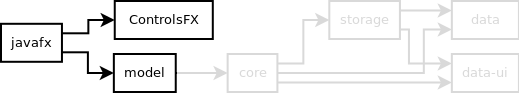
\includegraphics[width=.8\textwidth]{module_dependencies_javafx.png}
\end{figure}
\depBox{\refLongP{\textModModel}, ControlsFX (ext. \cite{controlsfx})}

Modulerklräung hier




\subsection{\textModModel}
\label{\textModModel}
\begin{figure}[h!]
	\centering
	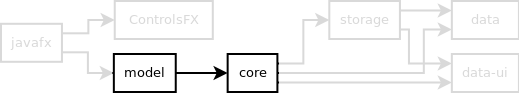
\includegraphics[width=.8\textwidth]{module_dependencies_model.png}
\end{figure}
\depBox{\refLongP{\textModCore}}

Dieses Modul wurde erst spät im Entwicklungsprozess mit einbezogen und beinhaltet bisher noch keine Klassen.
Es ist allerdings dafür vorgesehen, Klassen zu enthalten, die für die Oberfläche gebraucht werden, allerdings
unabhängig vom verwendeten Windowing-Toolkit sind.




\subsection{\textModStorage}
\label{\textModStorage}
\begin{figure}[h!]
	\centering
	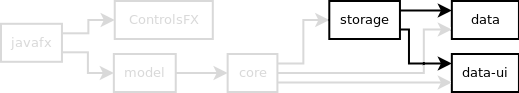
\includegraphics[width=.8\textwidth]{module_dependencies_storage.png}
\end{figure}
\depBox{\refLongP{\textModData}, \refLongP{\textModDataUI}}

Das Storage Modul enthält sowohl eine abstrake Definition von \textit{Serializern} und \textit{StorageHandlern}
als auch eine Implementation für XML inklusive \textit{Serializer} für Komponenten in \refLongP{\textModData} und
\refLongP{\textModDataUI}.

\subsubsection{StorageHandler}
Die Klasse \textit{StorageHandler} ist hält \textit{Storage}s und verteilt Serialisierungsaufgaben an
das entsprechende \textit{Storage} anhand eines Textidentifikators (für XML lautet dieser 'xml').
Eine weitere \textit{Storage} Implementation kann anhand eines neuen Textidentifkators registriert werden,
wodurch ein Umstieg von XML auf JSON, SQL oder eine andere Implementation vereinfacht wird.

\subsubsection{Storage}
Ein \textit{Storage} stellt ein Speicherort für alle zum Projekt gehörenden Komponenten dar. Je nach
Implementation kann dies XML (implementiert), JSON, SQL oder andere sein (nicht implementiert). Bei einem
\textit{Storage} können \textit{Serializer} für weitere Komponenten registriert werden. Sowohl Lese- als
auch Schreibhandles und Hilfsklassen für die \textit{Serializer} werden über Generics in \textit{Storage}
definiert.

\subsubsection{Serializer}
Ein \textit{Serializer} hat die Aufgabe eine Komponente zu serialisieren und wieder zu deserialisieren.
Der Umfang eines \textit{Serializer}s sollte sich auf eine Komponente beziehen (siehe \refLong{\textPrincipleSingleResponsibility}).